% flashcards-title: Upright-fit schematic, not to scale
% flashcards-desc: A rigid box is drawn beside two shelf boards that form an open gap. A vertical double-headed arrow marks the box height, labeled 29 cm; another marks the gap height, labeled 31 cm. The drawing is not to scale: the box is drawn slightly taller than the gap.
\documentclass[dvisvgm,tikz,border=8pt]{standalone}
\usepackage{tikz}
\usetikzlibrary{arrows.meta,calc,positioning}
\definecolor{DeckInk}{HTML}{172A3A}
\definecolor{DeckAccent}{HTML}{176B87}
\definecolor{DeckWarm}{HTML}{D97706}
\definecolor{DeckMuted}{HTML}{667784}
\definecolor{DeckPaper}{HTML}{F7FAFC}
\tikzset{
  every node/.style={font=\sffamily, text=DeckInk},
  object/.style={draw=DeckInk, line width=1.1pt, fill=DeckPaper},
  primary/.style={draw=DeckAccent, line width=1.5pt},
  boundary/.style={draw=DeckAccent, line width=1.5pt, dashed, rounded corners=6pt},
  guide/.style={draw=DeckMuted, line width=0.9pt, dashed},
  dimension/.style={{Stealth[length=3.2mm,width=2.2mm]}-{Stealth[length=3.2mm,width=2.2mm]}, draw=DeckWarm, line width=1.2pt},
  motion/.style={-{Stealth[length=3.5mm,width=2.5mm]}, draw=DeckAccent, line width=1.5pt, dashed},
}

\begin{document}
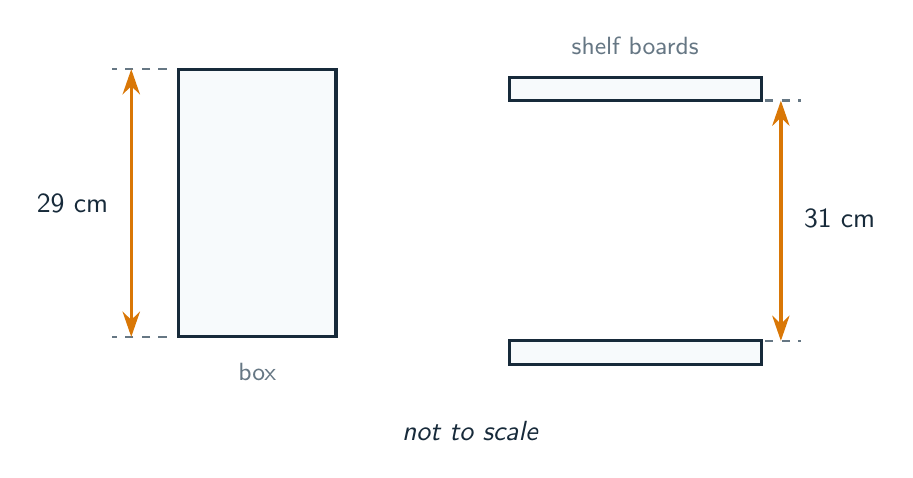
\begin{tikzpicture}[x=1cm,y=1cm]
  % Box (deliberately drawn slightly taller than the gap)
  \draw[object] (0,0) rectangle (2,3.4);
  \node[text=DeckMuted, font=\sffamily\small] at (1,-0.45) {box};

  % Box height dimension arrow with extension guides
  \draw[guide] (-0.15,0) -- (-0.85,0);
  \draw[guide] (-0.15,3.4) -- (-0.85,3.4);
  \draw[dimension] (-0.6,0) -- (-0.6,3.4);
  \node[text=DeckInk, font=\sffamily, left=2pt] at (-0.7,1.7) {29 cm};

  % Shelf boards forming the gap
  \draw[object] (4.2,-0.35) rectangle (7.4,-0.05);
  \draw[object] (4.2,3.0) rectangle (7.4,3.3);
  \node[text=DeckMuted, font=\sffamily\small] at (5.8,3.7) {shelf boards};

  % Gap height dimension arrow with extension guides
  \draw[guide] (7.45,-0.05) -- (7.9,-0.05);
  \draw[guide] (7.45,3.0) -- (7.9,3.0);
  \draw[dimension] (7.65,-0.05) -- (7.65,3.0);
  \node[text=DeckInk, font=\sffamily, right=2pt] at (7.75,1.5) {31 cm};

  % Not-to-scale note
  \node[text=DeckInk, font=\sffamily\itshape] at (3.7,-1.2) {not to scale};
\end{tikzpicture}
\end{document}
